
\chapter{学内ゾーンにおけるElasticsearchクラスタへのデータ移行}
\label{chap:second}

\section{緒言}
本章では学内ゾーンで稼働している Elasticsearch クラスタへのデータ移行について述べる.

\section{Elasticsearchの概要}
Elasticsearchは、分散処理に対応した全文検索エンジンである。主な特徴は、以下の通りである。

\begin{itemize}
    \item 高速な検索性能: ビッグデータなどの巨大で複雑なデータの集合にも対応可能
    \item 部分一致検索が可能: 検索キーワードの一部に一致するドキュメントも検索可能
    \item ほぼリアルタイムの検索: ドキュメントにインデックスを付けてから検索可能になるまで約1秒程度
    \item スケーラビリティ: サーバー数を増やすことで、検索性能と処理能力を拡張可能
\end{itemize}

これらの特徴から、Elasticsearchは、以下のような用途に適している。

\begin{itemize}
    \item ログ分析: Webサイトやアプリケーションのログから、アクセス状況やエラー情報を分析する
    \item セキュリティインテリジェンス: ネットワークやシステムから、セキュリティ脅威を検知する
    \item ビジネス分析: 顧客データや販売データから、トレンドや傾向を分析する
\end{itemize}

\section{kibanaの概要}

Kibanaは、Elasticsearchに保存されたデータを可視化するためのツールである。主な特徴は、以下の通りである。

\begin{itemize}
    \item 直感的な操作性: ドラッグ&ドロップで簡単に可視化を作成できる
    \item 豊富な可視化機能: グラフ、表、地図など、さまざまな可視化機能を提供
    \item 高度なフィルタリング機能: 条件を指定して、データを詳細に絞り込むことができる
\end{itemize}

これらの特徴から、Kibanaは、以下のような用途に適している。

\begin{itemize}
    \item ログ分析: Webサイトやアプリケーションのログから、アクセス状況やエラー情報を可視化する
    \item セキュリティインテリジェンス: ネットワークやシステムから、セキュリティ脅威を可視化する
    \item ビジネス分析: 顧客データや販売データから、トレンドや傾向を可視化する
\end{itemize}

\section{学内ゾーンで稼働しているElasticsearchシステムの状況}
学内ゾーンでは, 133.71.106.168で単一ノードのElasticsearchと, 133.71.106.170, 133.71.106.141, 133.71.106.136のElasticsearchノードによって構成されたElasticsearchクラスタが稼働している.

133.71.106.168のElasticsearchには, CO\textsubscript{2}濃度監視システムによって計測されたデータとLEAFの運行日誌に関するデータが保存されている.

\section{CO\textsubscript{2}濃度監視システムの概要}
CO\textsubscript{2}濃度監視システムとは共通講義棟 C, 工学部 5 号館,工学部 4 号館の各講義室(計 24 部屋)の CO2 濃度を学内ネットワーク内の web サイトで閲覧することができるシステムである.

Elasticsearchに保存されたデータには, 計測した日時, 部屋番号, 部屋の気温, CO\textsubscript{2}濃度などの情報が含まれている.

\section{データ移行対象のElasticsearchインデックスについて}

133.71.106.168で稼働している単一ノードのElasticsearchに保存されたCO\textsubscript{2}データとLEAFの運行日誌に関するデータを, 学内ゾーンで稼働しているElasticsearchクラスタへ移行する.

\section{CO\textsubscript{2}データの移行手順について}

CO\textsubscript{2}のデータ移行を行う上で, タイムスタンプと部屋番号の組み合わせが重複しているデータが一部存在しており, この重複データを取り除いた上でデータ移行を行う必要がある. そこで一度, 移行元のElasticSearchサーバーのデータをローカルマシンにエクスポートして, 重複データを取り除いた上で, 移行先のElasticSearchサーバーにデータをインサートする.

\subsection{データのエクスポート}
移行元のElasticSearchサーバーのデータのローカルマシンへのエクスポートには, elasticdumpライブラリを使用して, JSON形式でエクスポートした.その際, co2という文字列を含むインデックスのデータのみをエクスポートした.

\subsection{データの重複削除}
重複データの削除はSQLiteデータベースを用いて行った.

SQLiteデータベースはリレーショナルデータベースの一種であり, 複合主キーを使って複数のテーブルカラムの組み合わせを一意の識別子として扱うことができる. これにより, 同じ組み合わせのデータを重複して挿入しようとした場合, データベースエンジンがコンフリクトエラーを発生させ, 重複データの挿入を阻止する. そのため, 今回の重複データ削除には適していると判断した.

今回使用したSQLiteデータベースでは, 部屋番号(number)とタイムスタンプ(utctime)を一意のキーとして設定した. 以下のリスト\ref{sc1}, リスト\ref{sc2}に示すように, 移行元のElasticSearchサーバーに保存されているco2インデックスのドキュメントは, フィールドのメンバーが統一されておらず, 一部センサー情報が存在しない場合がある. そのため, データの挿入時にコンフリクトエラーが発生した場合は, 既存のレコードと挿入しようとしたレコードを比較し, 既存レコードの値がNULLであるカラムにおいて, 挿入しようとしているレコードの値が非NULLである場合には, 既存レコードのカラムの値を更新するようにした. これにより, 重複データ削除時に一部センサー情報などが欠けてしまう問題を解決した.

\begin{lstlisting}[caption=\_sourceフィールドのメンバー数が少ないドキュメント, label=sc1]
{
  "_index": "co2_e411",
  "_type": "_doc",
  "_id": "nEi2nnoB2-iFXnrMOobM",
  "_score": 1,
  "_source": {
      "utctime": "2020-10-09T05:09:06+00:00",
      "number": "E411",
      "PPM": "481",
      "data": "Thingspeak"
  }
}
  \end{lstlisting}

\begin{lstlisting}[caption=\_sourceフィールドのメンバー数が多いドキュメント, label=sc2]
{
  "_index": "co2_e411",
  "_type": "_doc",
  "_id": "YKBqU4QBugDzeydA2gyi",
  "_score": 1,
  "_source": {
      "RH": 26.98,
      "PPM": 423,
      "JPtime": "2022-11-06T22:45:30.080925",
      "ip": "172.23.68.19/16",
      "utctime": "2022-11-06T13:45:30.080895",
      "TEMP": 24.47,
      "index_name": "co2_e411",
      "ms": "",
      "number": "E411"
  }
}
    \end{lstlisting}

\subsection{データのインポート}
重複データ削除後のデータが保存されたSQLiteテーブルからすべてのレコードを読み出して, ターゲットのElasticSearchサーバーに移行した.

その際, pythonのelasticsearchライブラリを使用し, co2\_modbusという名前のインデックスに保存した.

\section{一度目のデータ移行で移行できなかったCO\textsubscript{2}データの移行について}

実装したデータ移行プログラムを使用して133.71.201.197から133.71.106.141のElasticSearchサーバーへCO\textsubscript{2}データを移行したのが2023年5月中旬頃であり, CO\textsubscript{2}濃度監視システムを開発, 運用している高木君が, 移行先である133.71.106.141のElasticSearchサーバーに対してラズベリーパイからCO\textsubscript{2}データのインサートを行うよう対応したのが2023年7月中旬であったため, 2023年5月中旬から2023年7月中旬までの間の約2ヶ月間のCO\textsubscript{2}データが移行先のElasticSearchサーバーに移行出来ていなかった. そこで, 追加の移行作業を行った.

移行方法は以下のとおりである.

\begin{enumerate}
    \item まず, 2023年5月中旬に移行した際の全移行データの中で最も最新のutctimeフィールドの値を検索する.
          \begin{itemize}
              \item 検索した結果, 2023年5月中旬に移行した際の全移行データの中で最も最新のutctimeは「2023-05-16T05:48:30.081305」であった.
          \end{itemize}
    \item 次に, 移行先ElasticSearchサーバーに対してラズベリーパイからインサートされた全データの中で最も古いutctimeフィールドの値を検索する.
          \begin{itemize}
              \item 検索した結果, ラズベリーパイからインサートされた全データの中で最も古いutctimeは「2023-07-20T07:15:39.314008」であった.
          \end{itemize}
    \item 前回のCO\textsubscript{2}データの移行は2023年5月中旬頃に行ったため, 2023年5月1日0時0分0秒以降のutctimeを持つドキュメントを, 移行元ElasticSearchサーバーのインデックス名にco2という文字列を含むインデックスからelasticdump \cite{1}ライブラリを使用してローカルマシンにエクスポートする.
    \item 部屋番号(number)とタイムスタンプ(utctime)の組み合わせがユニークになるようにエクスポートしたデータをフィルタリングする.
    \item 更に, 1と2で得られたutctimeの範囲に含まれるutctimeを持つドキュメントのみになるようフィルタリングする.
    \item フィルタリング後のデータを移行先ElasticSearchサーバーにバルクインサートする.
\end{enumerate}

\section{kibanaによるデータの可視化}

計2回のCO\textsubscript{2}データを移行した後のco2\_modbusインデックスについて, 横軸をタイムスタンプ(utctime)とし, 縦軸をPPM, RH, TEMPとしてそれぞれプロットしたものを図 \ref{p12} 〜 図 \ref{p14}に示す.

\begin{figure}
    \begin{center}
        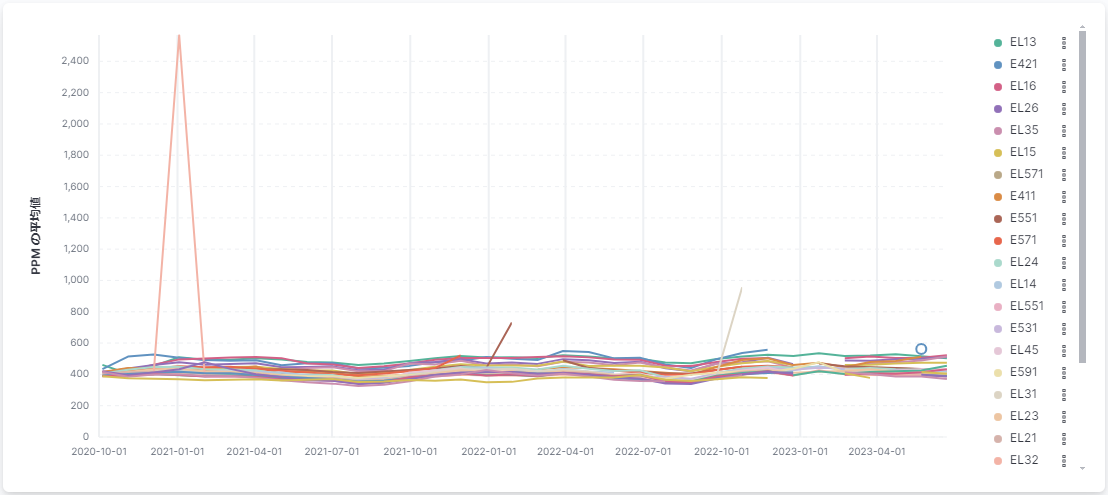
\includegraphics[width=160mm]{sotu/figure/ppm.png}
        \caption{co2\_modbusのPPM}
        \label{p12}
    \end{center}
\end{figure}

\begin{figure}
    \begin{center}
        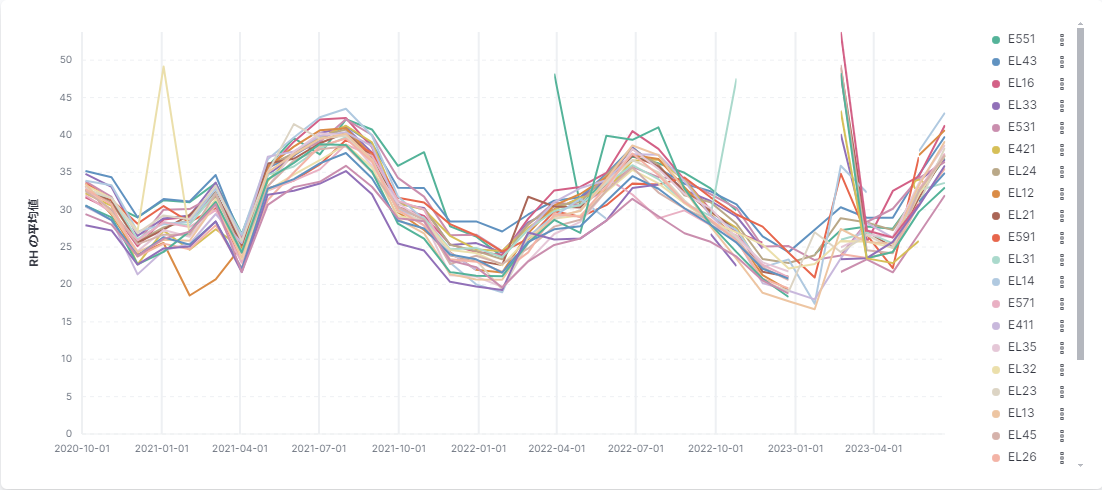
\includegraphics[width=160mm]{sotu/figure/rh.png}
        \caption{co2\_modbusのRH}
        \label{p13}
    \end{center}
\end{figure}

\begin{figure}
    \begin{center}
        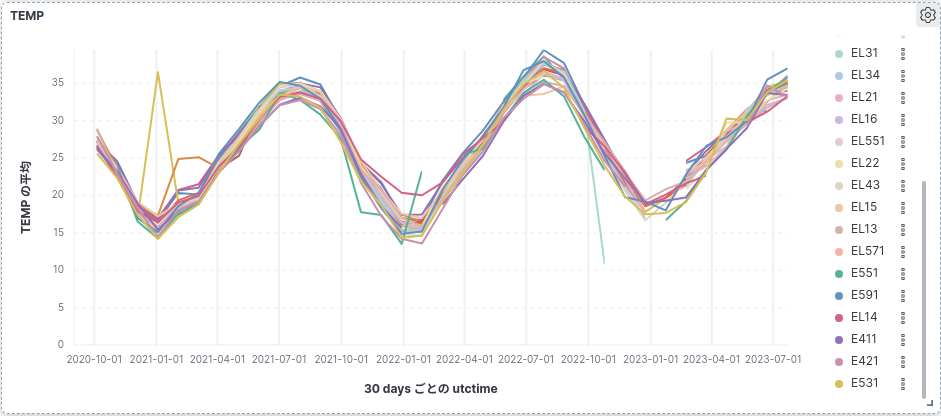
\includegraphics[width=160mm]{sotu/figure/temp.png}
        \caption{co2\_modbusのTEMP}
        \label{p14}
    \end{center}
\end{figure}

2回目のCO\textsubscript{2}データの移行によって, 2023年5月中旬から2023年7月中旬までの期間とその前後の期間において, 図 \ref{p12} 〜 図 \ref{p14}より, 連続的にデータが変化していることが目視で確認できるので, データ移行は正常に出来たと判断できる.

\section{LEAFの運行日誌に関するデータの移行について}

LEAFの運行日誌に関するデータが保存されたインデックスは以下の2つである.

\begin{itemize}
    \item movement\_diary
    \item movement\_diary01
\end{itemize}

これらのインデックスのデータ移行は, 同名のインデックスを移行先のElasticSearchサーバーに作成して, 作成したインデックスにデータを挿入することで行った.

次に, 上記のインデックスに保存されているデータについて説明する.

以下にmovement\_diaryとmovement\_diary01のドキュメントの違いを列挙する.

\begin{enumerate}
    \item driverフィールド:
          \begin{itemize}
              \item movement\_diaryのドキュメントでは, driverフィールドは文字列である.
              \item movement\_diary01のドキュメントでは, driverフィールドは配列で, その中に文字列と2つのnull値が含まれている.
          \end{itemize}
          
    \item ``destination''フィールド:
          \begin{itemize}
              \item movement\_diaryのドキュメントでは, ``destination''フィールドは単一の文字列である.
              \item movement\_diary01のドキュメントでは, ``destination''フィールドは配列で, その中に2つの文字列が含まれている.
          \end{itemize}
          
    \item ``charge\_place''フィールド:
          \begin{itemize}
              \item movement\_diaryのドキュメントには, ``charge\_place''フィールドは存在しない.
              \item movement\_diary01のドキュメントでは, ``charge\_place''フィールドが追加されているが, その値は空文字列である.
          \end{itemize}
          
    \item ``battery\_rate''フィールド:
          \begin{itemize}
              \item movement\_diaryのドキュメントには, ``battery\_rate''フィールドは存在しない.
              \item movement\_diary01のドキュメントでは, ``battery\_rate''フィールドが追加されており, その値は数値である.
          \end{itemize}
          
    \item ``battery\_rate\_distance''フィールド:
          \begin{itemize}
              \item movement\_diaryのドキュメントには, ``battery\_rate\_distance''フィールドは存在しない.
              \item movement\_diary01のドキュメントでは, ``battery\_rate\_distance''フィールドが追加されており, その値は数値である.
          \end{itemize}
\end{enumerate}

movement\_diaryとmovement\_diary01のドキュメントの違いより, movement\_diary01はmovement\_diaryのもつ情報量を全て保持しており, その上で追加のフィールドを持っていることから, 移行するのはmovement\_diary01インデックスのみで十分であることが分かった.

\section{LEAFの運行日誌に関するデータの移行手順について}

\subsection{データのエクスポート}
移行元のElasticSearchサーバーのデータのローカルマシンへのエクスポートには, elasticdumpライブラリを使用して, movement\_diary01インデックスの全ドキュメントをJSON形式でエクスポートした.

\subsection{データのインポート}
pythonのelasticsearchライブラリを使用し, 移行先のElasticsearchにmovement\_diary01という名前のインデックスを作成して, エクスポートしたデータを全てインサートした.

\section{結言}
本章学内ゾーンで稼働している Elasticsearch クラスタへのデータ移行について述べた。

次章ではサーバーゾーンでのクラスタ構築における仮想環境を使用した事前検証について述べる。